\documentclass[handout]{beamer}

\usepackage{fontspec} 
% \usepackage{lsp-makros}
\useoutertheme{lsp}

\usepackage{lsptitle}

\def\two@digits#1{\ifnum#1<10 0\fi\number#1}
\def\mytoday{\two@digits{\number\day}.\two@digits{\number\month}.\number\year}


\usepackage{xspace,multicol}
\newcommand{\latex}{\LaTeX\xspace}
\usepackage{tikz}


\newcounter{lastpagemainpart}
\footnotesep0pt
\renewcommand{\footnoterule}{}
\usefootnotetemplate{
  \noindent
  \insertfootnotemark\insertfootnotetext}

\let\beamerfn=\footnote
\renewcommand{\footnote}[1]{%
\let\oldfnsize=\footnotesize%
\let\footnotesize=\tiny%
\beamerfn<\thebeamerpauses->{#1}%
\let\footnotesize=\oldfnsize}


\date{\today}

\usepackage{eurosym}  
 
\renewcommand{\centerline}[1]{\hfill#1\hfill\hfill\mbox{}}


\title{Proofreading}
% \institute{FU Berlin}
\author[LangSci]{Language Science Press}



\begin{document}
\lspbeamertitle

\section{Proofreading}
\frame{
\frametitle{Workflow}
%   \includegraphics[height=.2\textheight]{./path/to/graphicsfile}
  \begin{enumerate}
    \item prepare manuscript
    \item compile mail
    \item retrieve registered proofreader addresses (ca. 400)
    \item remove blacklisted proofreaders (9)
    \item announce new book to proofreaders
    \item collect volunteers
    \item upload proofreading pdf to PaperHive
    \item assign chapters and inform volunteers
    \item wait
    \item check coverage
    \item forward
  \end{enumerate}
}

\frame{
\frametitle{PaperHive}
  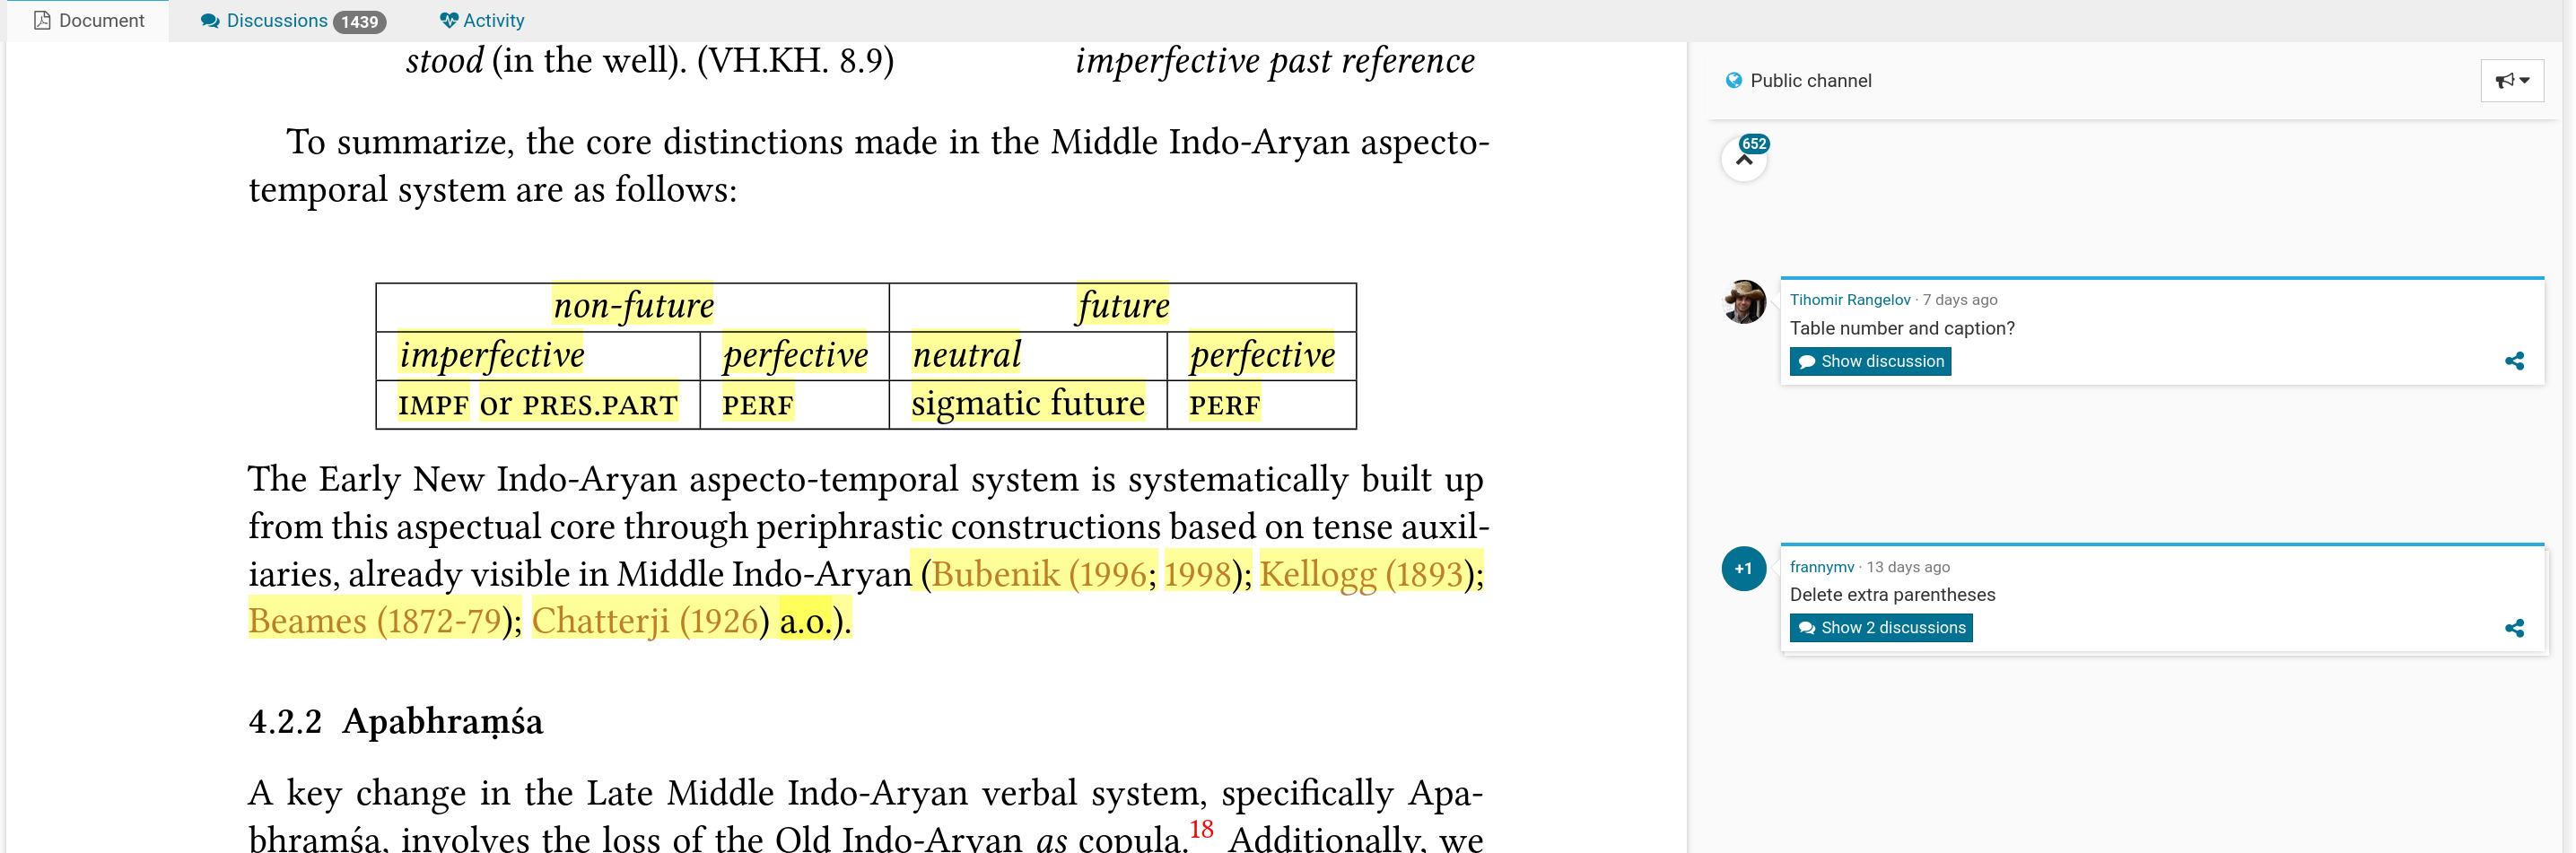
\includegraphics[width=1.05\textwidth]{proofreading.png}
}

\frame{
\frametitle{Differences to traditional\strut\newline proofreading}
%   \includegraphics[height=.2\textheight]{./path/to/graphicsfile}
  \begin{itemize}
    \item quantitative
    \begin{itemize}
      \item 2.6 comments/page at LangSci
    \end{itemize}
    \item qualitative
    \begin{itemize}
      \item      more content, less style matters
      \item      not everybody is a native speaker
      \item      not everybody is a trained proofreader
      \item      all comments have to be taken with a grain of salt
      \item      advantage: all comments show that someone had some problem understanding what was written (even if grammatically technically correct)
    \end{itemize}
  \end{itemize}
}

%\setcounter{framenumber}{\thelastpagemainpart}
\end{document}
